% Cardiac EP forward pipeline + single-level Schwarz preconditioning study.
% Minimal academic style, English.  Compile with: pdflatex (x2) or xelatex (x2).
\documentclass[aspectratio=169,10pt]{beamer}
\usepackage[T1]{fontenc}
\usepackage{lmodern}
\usepackage{amsmath,amssymb,bm}
\usepackage{booktabs}
\usepackage{array}
\usepackage{tikz}
\usetikzlibrary{arrows.meta,positioning}

\definecolor{Struct}{HTML}{1F3A5F}
\definecolor{Gray}{HTML}{6E6E6E}
\definecolor{Accent}{HTML}{8C2D04}

\usetheme{default}
\usefonttheme{professionalfonts}
\setbeamertemplate{navigation symbols}{}
\setbeamercolor{structure}{fg=Struct}
\setbeamercolor{frametitle}{fg=Struct}
\setbeamerfont{frametitle}{series=\bfseries,size=\large}
\setbeamercolor{normal text}{fg=black}
\setbeamertemplate{itemize item}{\textbullet}
\setbeamertemplate{itemize subitem}{--}
\setbeamercolor{block title}{fg=white,bg=Struct}
\setbeamercolor{block body}{bg=Struct!6}
\setbeamertemplate{frametitle}{\vskip0.45em\hspace{0.2em}\usebeamerfont{frametitle}\insertframetitle%
  {\ifx\insertframesubtitle\empty\else\\[0.1em]\small\color{Gray}\insertframesubtitle\fi}\par}
\setbeamertemplate{footline}{\hfill\footnotesize\color{Gray}\insertframenumber\,/\,\inserttotalframenumber\hspace{0.4cm}\vspace{3pt}}
\renewcommand{\arraystretch}{1.15}

% ---- consistent notation macros (used everywhere) ----
\newcommand{\Vm}{V_{\mathrm m}}
\newcommand{\ue}{u_{\mathrm e}}
\newcommand{\uT}{u_{\mathrm T}}
\newcommand{\Iion}{I_{\mathrm{ion}}}
\newcommand{\Istim}{I_{\mathrm{stim}}}
\newcommand{\Cm}{C_{\mathrm m}}
\newcommand{\sm}{\bm\sigma_{\mathrm m}}
\newcommand{\si}{\bm\sigma_{\mathrm i}}
\newcommand{\se}{\bm\sigma_{\mathrm e}}
\newcommand{\sT}{\sigma_{\mathrm T}}
\newcommand{\OH}{\Omega_{\mathrm H}}
\newcommand{\OT}{\Omega_{\mathrm T}}
\newcommand{\nn}{\mathbf n}
\newcommand{\Mmat}{\mathbf M}
\newcommand{\Kmat}{\mathbf K}
\newcommand{\ww}{\bm w}
\newcommand{\zz}{\bm z}
\newcommand{\Vvec}{\mathbf V}
\newcommand{\uevec}{\mathbf u_{\mathrm e}}
\newcommand{\uTvec}{\mathbf u_{\mathrm T}}

\begin{document}

% ===== Title =====
\begin{frame}[plain]
  \vskip0.9cm
  {\color{Struct}\large\bfseries A Cardiac Electrophysiology Forward Pipeline\\[0.25em]
   and Single-Level Schwarz Preconditioning\par}
  \vskip0.5em
  {\color{Gray} Continuous \& discrete formulation $\;\cdot\;$ the overlap anomaly $\;\cdot\;$ cross-system preconditioning\par}
  \vskip0.9em\hrule height0.4pt\vskip0.7em
  \footnotesize
  Part I--II: ionic model $\to$ monodomain $\to$ extracellular recovery $\to$ torso (real geometry).\\[0.2em]
  Part III: overlap-dependent CG iteration growth in ASM\,+\,ICC (abstract test problems).\\[0.2em]
  Part IV: can one system precondition another? --- theory, prior art, and transferable ideas.\\[0.4em]
  Code \& data: \texttt{github.com/tianhaomahpc-ops/cg-asm-icc-research}
\end{frame}

% ===================================================================
% PART I  --  CONTINUOUS PROBLEM
% ===================================================================
\begin{frame}{Part I --- Continuous problem: domains and notation}
\begin{columns}[T]
\begin{column}{0.46\textwidth}
\centering
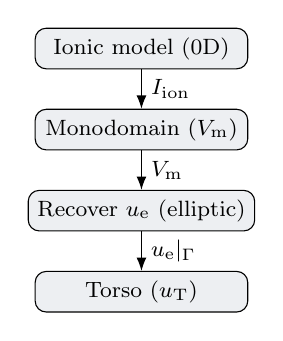
\begin{tikzpicture}[font=\footnotesize,>=Latex,node distance=5mm]
\node[draw,rounded corners,fill=Struct!8,minimum width=2.7cm] (ion){Ionic model (0D)};
\node[draw,rounded corners,fill=Struct!8,below=of ion,minimum width=2.7cm] (mono){Monodomain ($\Vm$)};
\node[draw,rounded corners,fill=Struct!8,below=of mono,minimum width=2.7cm] (ue){Recover $\ue$ (elliptic)};
\node[draw,rounded corners,fill=Struct!8,below=of ue,minimum width=2.7cm] (torso){Torso ($\uT$)};
\draw[->] (ion)--(mono) node[midway,right]{$\Iion$};
\draw[->] (mono)--(ue) node[midway,right]{$\Vm$};
\draw[->] (ue)--(torso) node[midway,right]{$\ue|_\Gamma$};
\end{tikzpicture}
\vskip0.3em
{\footnotesize Heart $\OH$ and torso $\OT$ are \emph{two meshes sharing} the heart surface $\Gamma=\partial\OH$.}
\end{column}
\begin{column}{0.54\textwidth}
\scriptsize\setlength{\tabcolsep}{3pt}
\begin{tabular}{@{}ll@{}}
\toprule
$\Vm,\ue$ & transmembrane / extracellular potential (in $\OH$) \\
$\uT$ & torso potential (in $\OT$) \\
$\ww,\zz$ & gating variables / ion concentrations \\
$\Iion,\Istim$ & total ionic current / stimulus current \\
$\chi,\Cm$ & surface-to-volume ratio, membrane capac. \\
$\si,\se,\sm$ & intra / extra / monodomain conductivities \\
$\sT$ & torso conductivity (uniform scalar) \\
$\Gamma,\,\partial\OT^{\mathrm{ext}}$ & heart--torso interface, body surface \\
$\Mmat,\Kmat_{\bm\sigma}$ & P1 mass / stiffness ($\bm\sigma$-weighted) \\
$\Delta t,\,n$ & time step ($0.01$\,ms), time index \\
\bottomrule
\end{tabular}
\end{column}
\end{columns}
\vskip0.4em
{\footnotesize Parameters: Niederer et al.\ (2011) benchmark; cell model: ten~Tusscher--Panfilov (2006, ``TP06'').}
\end{frame}

% ---- S2 ionic ----
\begin{frame}{1. Ionic model (TP06, 0D cell kinetics)}
\framesubtitle{state split into gating variables $\ww$ and concentrations $\zz$ (the only ODEs written here)}
At each spatial point, the membrane current is governed by gating and concentration ODEs:
\[
\textbf{gating:}\ \ \dot w_j=\frac{w_{j,\infty}(\Vm)-w_j}{\tau_{w_j}(\Vm)},
\quad
\textbf{concentrations:}\ \ \dot z_k=f_{z_k}(\Vm,\ww,\zz),
\]
with the total ionic current assembled from the TP06 channel/pump/exchanger currents
\[
\Iion=\Iion(\Vm,\ww,\zz).
\]
\begin{itemize}\itemsep0.3em
  \item $\ww$ = voltage-gated gating variables (Hodgkin--Huxley form, hence the $w_\infty,\tau_w$ structure).
  \item $\zz$ = intracellular ionic concentrations (and related state).
  \item In tissue, $\Vm$ is \emph{not} a 0D ODE: it is advanced by the monodomain PDE (next slide); $\Iion$ enters that PDE as the reaction term.
  \item Sign convention and rate functions: as in the TP06 model with Niederer-benchmark parameters.
\end{itemize}
\end{frame}

% ---- S3 monodomain ----
\begin{frame}{2. Monodomain equation (reaction--diffusion for $\Vm$)}
\framesubtitle{in the heart $\OH$, with an electrically insulated surface}
\[
\boxed{\;\chi\Big(\Cm\,\frac{\partial \Vm}{\partial t}+\Iion(\Vm,\ww,\zz)\Big)
=\nabla\!\cdot(\sm\nabla \Vm)+\Istim\;}\qquad\text{in }\OH\times(0,T]
\]
\[
\textbf{boundary condition:}\qquad (\sm\nabla \Vm)\cdot\nn=0 \quad\text{on }\partial\OH=\Gamma
\quad(\text{no extracellular coupling}).
\]
\begin{itemize}\itemsep0.3em
  \item $\sm=\si(\si+\se)^{-1}\se$ : monodomain conductivity (harmonic combination of intra/extra).
  \item $\chi,\Cm,\sm$ : Niederer et al. (2011) benchmark values (anisotropic, fiber-aligned $\sm$).
  \item $\Istim$ : applied stimulus (location / waveform omitted here by request).
  \item Coupled to the cell model through $\Iion$; this is the parabolic stage of the pipeline.
\end{itemize}
\end{frame}

% ---- S4 recover ue ----
\begin{frame}{3. Recover the extracellular potential $\ue$}
\framesubtitle{elliptic problem in the heart $\OH$ --- pure Neumann, singular}
\[
\boxed{\;-\nabla\!\cdot\big((\si+\se)\nabla \ue\big)=\nabla\!\cdot(\si\nabla \Vm)\;}\qquad\text{in }\OH
\]
\[
\textbf{boundary condition (pure Neumann):}\qquad
\big((\si+\se)\nabla \ue\big)\cdot\nn=-(\si\nabla \Vm)\cdot\nn\quad\text{on }\Gamma .
\]
\begin{itemize}\itemsep0.3em
  \item Operator $-\nabla\!\cdot((\si+\se)\nabla\,\cdot\,)$ with all-Neumann data is \textbf{singular}: $\ker=\{\text{constants}\}$.
  \item Solvability: the right-hand side must have zero mean over $\OH$ (current balance); the solution is fixed by the \textbf{mean-zero gauge} $\int_{\OH}\ue=0$.
  \item This is the elliptic ``bidomain-recovery'' stage; $\Vm$ from stage~2 is its data.
  \item In the linear-algebra study (Part III) this is the prototype of the \emph{singular all-Neumann} system.
\end{itemize}
\end{frame}

% ---- S5 torso ----
\begin{frame}{4. Torso model (passive volume conductor)}
\framesubtitle{elliptic problem in the torso $\OT$ --- one-way coupling from the heart}
\[
\boxed{\;-\nabla\!\cdot(\sT\nabla \uT)=0\;}\qquad\text{in }\OT,\qquad \sT=\text{const (uniform)}
\]
\[
\textbf{coupling (Dirichlet, one-way):}\ \ \uT=\ue\ \ \text{on }\Gamma;
\qquad
\textbf{body surface:}\ \ (\sT\nabla \uT)\cdot\nn=0\ \ \text{on }\partial\OT^{\mathrm{ext}}.
\]
\begin{itemize}\itemsep0.3em
  \item One-way: the heart supplies $\ue|_\Gamma$ as \textbf{Dirichlet} data; no feedback to the heart.
  \item Mixed BC (Dirichlet on $\Gamma$, Neumann on the body surface) $\Rightarrow$ \textbf{non-singular} elliptic solve.
  \item $\OH$ and $\OT$ are two meshes that share the surface $\Gamma$; $\ue|_\Gamma$ is transferred across the conforming interface.
  \item Prototype (Part III) of the \emph{mixed Dirichlet/Neumann} system (well-posed, ill-conditioned).
\end{itemize}
\end{frame}

% ===================================================================
% PART II  --  DISCRETE PROBLEM
% ===================================================================
\begin{frame}{Part II --- Discretization: common setup}
\begin{itemize}\itemsep0.4em
  \item \textbf{Space:} P1 (piecewise-linear) finite elements on tetrahedral meshes $\mathcal T_h$ of $\OH$ and $\OT$; nodal unknowns.
  \item \textbf{Matrices} (per domain / conductivity):
  \[
  (\Mmat)_{ab}=\!\int \varphi_a\varphi_b,\qquad
  (\Kmat_{\bm\sigma})_{ab}=\!\int \bm\sigma\nabla\varphi_a\cdot\nabla\varphi_b
  \quad(\text{SPD, }\ \Kmat_{\bm\sigma}\leftrightarrow -\nabla\!\cdot(\bm\sigma\nabla\,\cdot)).
  \]
  \item \textbf{Time:} $\Delta t=0.01$\,ms; superscript $n$ denotes time level $t_n=n\Delta t$.
  \item \textbf{Splitting (IMEX):} the diffusion is treated implicitly (Crank--Nicolson), the reaction $\Iion$ as an \textbf{explicit source}; the gating/concentration ODEs are integrated pointwise.
  \item \textbf{Initial conditions:} $\Vm^0=-83$\,mV (resting), $\ww^0,\zz^0=$ TP06 resting state, $\ue^0=0$, $\uT^0=0$.
\end{itemize}
\end{frame}

% ---- S7 ionic integration ----
\begin{frame}{1$'$. Ionic time integration: Rush--Larsen + forward Euler}
\framesubtitle{pointwise at every node, advancing $t_n\to t_{n+1}$ from $\Vm^n$}
\textbf{Gating $\ww$ --- Rush--Larsen} (exact for the frozen-$\Vm$ linear ODE; unconditionally stable):
\[
w_j^{n+1}=w_{j,\infty}(\Vm^n)+\big(w_j^{n}-w_{j,\infty}(\Vm^n)\big)\,\exp\!\Big(\!-\frac{\Delta t}{\tau_{w_j}(\Vm^n)}\Big).
\]
\textbf{Concentrations $\zz$ --- forward Euler:}
\[
z_k^{n+1}=z_k^{n}+\Delta t\,f_{z_k}(\Vm^n,\ww^{n},\zz^{n}).
\]
\textbf{Explicit ionic current} (the source fed to the monodomain solve):
\[
\Iion^{n}:=\Iion(\Vm^{n},\ww^{n+1},\zz^{n+1}).
\]
\vskip0.3em
{\footnotesize Rush--Larsen handles the stiff gating kinetics; forward Euler suffices for the slower concentrations.}
\end{frame}

% ---- S8 monodomain discrete = Sys1 ----
\begin{frame}{2$'$. Monodomain: Crank--Nicolson diffusion, explicit reaction \;$\Rightarrow$\; \textbf{Sys\,1}}
\framesubtitle{P1 FEM in space; the reaction $\Iion^n$ is a known right-hand side}
\[
\boxed{\;\underbrace{\Big(\tfrac{\chi\Cm}{\Delta t}\Mmat+\tfrac12\Kmat_{\sm}\Big)}_{\textstyle \mathbf A_1\ (\text{SPD})}\Vvec^{n+1}
=\Big(\tfrac{\chi\Cm}{\Delta t}\Mmat-\tfrac12\Kmat_{\sm}\Big)\Vvec^{n}-\chi\,\Mmat\,\Iion^{n}+\Mmat\,\Istim^{n}\;}
\]
\begin{itemize}\itemsep0.3em
  \item \textbf{Sys\,1} $=\mathbf A_1=\tfrac{\chi\Cm}{\Delta t}\Mmat+\tfrac12\Kmat_{\sm}$ --- the matrix our study calls $\tfrac1{\Delta t}M+\tfrac12K$.
  \item At $\Delta t=0.01$\,ms the \textbf{mass term dominates} $\Rightarrow$ well-conditioned $\Rightarrow$ very few CG iterations.
  \item Explicit reaction keeps the left-hand side \emph{linear, SPD, and constant in time} $\Rightarrow$ the preconditioner is built once and reused every step.
\end{itemize}
\end{frame}

% ---- S9 recover ue discrete = Sys2 ----
\begin{frame}{3$'$. Recover $\ue$: P1 FEM \;$\Rightarrow$\; \textbf{Sys\,2} (singular)}
\[
\boxed{\;\Kmat_{\si+\se}\,\uevec^{\,n+1}=-\,\Kmat_{\si}\,\Vvec^{n+1}\;}
\qquad\text{then re-gauge}\quad \uevec^{\,n+1}\leftarrow \uevec^{\,n+1}-\mathrm{mean}(\uevec^{\,n+1}).
\]
\begin{itemize}\itemsep0.3em
  \item \textbf{Sys\,2} $=\Kmat_{\si+\se}$ : symmetric positive \emph{semi}-definite, $\ker=\mathrm{span}\{\mathbf 1\}$.
  \item Right-hand side $-\Kmat_{\si}\Vvec^{n+1}$ is consistent (in $\mathrm{range}$); the constant null mode is removed from the RHS and from the iterate (mean-zero gauge).
  \item Solved by preconditioned CG on the consistent singular system (no operator shift).
\end{itemize}
\end{frame}

% ---- S10 torso discrete ----
\begin{frame}{4$'$. Torso: P1 FEM with interface Dirichlet data \;$\Rightarrow$\; \textbf{Sys\,3}-type}
\[
\boxed{\;\Kmat_{\sT}\,\uTvec^{\,n+1}=\mathbf 0\;}\qquad
\text{subject to}\quad \uTvec^{\,n+1}\big|_{\Gamma}=\Pi\big(\uevec^{\,n+1}\big|_{\Gamma}\big),
\]
with $(\sT\nabla\uT)\cdot\nn=0$ on the body surface $\partial\OT^{\mathrm{ext}}$.
\begin{itemize}\itemsep0.3em
  \item $\Pi$ : transfer of $\ue$ from the heart-surface trace to the torso mesh (shared $\Gamma$, conforming).
  \item Dirichlet rows on $\Gamma$ make the system \textbf{non-singular}; reduced operator is SPD.
  \item Mixed Dirichlet ($\Gamma$) / Neumann (body) $\Rightarrow$ the well-posed but ill-conditioned elliptic prototype studied abstractly in Part III.
\end{itemize}
\end{frame}

% ---- S11 full algorithm ----
\begin{frame}{One time step: the full update $t_n\to t_{n+1}$}
\begin{block}{Given $\Vm^n,\ww^n,\zz^n$ (and $\ue^n,\uT^n$):}
\footnotesize
\begin{enumerate}\itemsep0.25em
  \item[(1)] \textbf{Gating} (Rush--Larsen): $\ww^{n+1}\leftarrow$ exact exponential update from $\Vm^n$.
  \item[(2)] \textbf{Concentrations} (forward Euler): $\zz^{n+1}\leftarrow \zz^{n}+\Delta t\,f_{\zz}(\Vm^n,\ww^n,\zz^n)$.
  \item[(3)] \textbf{Ionic source} (explicit): $\Iion^{n}\leftarrow \Iion(\Vm^n,\ww^{n+1},\zz^{n+1})$.
  \item[(4)] \textbf{Monodomain} (Sys\,1): solve $\mathbf A_1\Vvec^{n+1}=\big(\tfrac{\chi\Cm}{\Delta t}\Mmat-\tfrac12\Kmat_{\sm}\big)\Vvec^{n}-\chi\Mmat\Iion^{n}+\Mmat\Istim^{n}$.
  \item[(5)] \textbf{Recover $\ue$} (Sys\,2): solve $\Kmat_{\si+\se}\uevec^{\,n+1}=-\Kmat_{\si}\Vvec^{n+1}$; re-gauge to mean zero.
  \item[(6)] \textbf{Torso} (Sys\,3): solve $\Kmat_{\sT}\uTvec^{\,n+1}=\mathbf 0$ with $\uTvec|_\Gamma=\Pi(\uevec^{\,n+1}|_\Gamma)$.
\end{enumerate}
\end{block}
\vskip0.2em
{\footnotesize \textbf{All four solves} are performed every step. The three linear systems (Sys\,1/2/3) share the heart mesh and sparsity; their matrices are constant in time, so each preconditioner is set up once and reused.}\\[0.2em]
{\footnotesize Initial conditions: $\Vm^0=-83$\,mV, $\ww^0,\zz^0=$ TP06 resting state, $\ue^0=\uT^0=0$.}
\end{frame}

% ===================================================================
% PART III  --  THE OVERLAP ANOMALY (abstract test problems)
% ===================================================================
\begin{frame}{Part III --- The overlap anomaly (abstract test problems)}
\framesubtitle{not the real geometry: clean prototypes that isolate the linear algebra}
\textbf{Solver under study:} CG $+$ additive Schwarz (\texttt{PCASM}, BASIC variant) $+$ subdomain ICC($L$), overlap $O$.
\vskip0.4em
\textbf{Prototype problems} on the unit cube $[0,1]^3$, P1 tetrahedra, $n_x{=}48$ ($117{,}649$ DOF), 4 MPI ranks, METIS:
\begin{itemize}\itemsep0.3em
  \item mixed Dirichlet/Neumann Laplace (1 Dirichlet $+$ 5 Neumann faces) --- analogue of the torso solve;
  \item all-Neumann singular Laplace ($\ker=\{\text{const}\}$) --- analogue of the $\ue$ recovery;
  \item reaction--diffusion $\tfrac1{\Delta t}\Mmat+\tfrac12\Kmat$ --- analogue of the monodomain step.
\end{itemize}
\vskip0.3em
\textbf{Expectation} (classical overlapping Schwarz, exact local solves): more overlap $\Rightarrow$ smaller condition number $\Rightarrow$ \emph{fewer} iterations.
\end{frame}

% ---- S13 anomaly ----
\begin{frame}{The suspicious result: more overlap $\Rightarrow$ \emph{more} iterations}
\framesubtitle{BASIC ASM $+$ CG, mixed-BC Laplace; CG iteration count}
\begin{center}\footnotesize\setlength{\tabcolsep}{5pt}
\begin{tabular}{c ccccccc}
\toprule
$O\backslash L$ & 0 & 1 & 2 & 3 & 4 & 5 & 6 \\
\midrule
0 & 132 & 102 & 87 & 77 & 72 & 66 & 64 \\
1 & 148 & 102 & 92 & 75 & 65 & 56 & 50 \\
2 & 179 & 117 & 90 & 74 & 65 & 57 & 51 \\
3 & 199 & 130 & 103 & 80 & 59 & 56 & 50 \\
\midrule
trend in $O$ & $\uparrow$ & $\uparrow$ & $\uparrow$ & $\approx$ & $\downarrow$ & $\downarrow$ & $\downarrow$ \\
\bottomrule
\end{tabular}
\end{center}
\vskip0.4em
\begin{itemize}\itemsep0.25em
  \item At low fill ($L{\le}3$): increasing overlap \textbf{raises} the iteration count ($132\to199$ at $L{=}0$) --- opposite to theory.
  \item The professor's objection: ``more overlap should help.'' It does --- but only once $L$ is large enough.
\end{itemize}
\end{frame}

% ---- S14 cause ----
\begin{frame}{Conjecture: two coupled causes}
\framesubtitle{the abstract Schwarz condition-number bound}
\[
\kappa(\mathbf B^{-1}\mathbf A)\ \le\
\underbrace{C_0^{2}}_{\substack{\text{stable splitting}\\ \delta\uparrow\Rightarrow\downarrow}}\ \cdot\
\underbrace{\omega}_{\substack{\text{(A) local solve}\\ \text{exact}{=}1,\ \text{ICC}{>}1}}\ \cdot\
\underbrace{N_c}_{\substack{\text{(B) overlap colouring}\\ \delta\uparrow\Rightarrow\uparrow}}
\qquad\text{(Toselli \& Widlund, Thm.\ 2.7)}
\]
\begin{itemize}\itemsep0.3em
  \item \textbf{(A) inexact subdomain solve.} ICC is not the exact block inverse: $\omega>1$, and it worsens as the overlapped block grows.
  \item \textbf{(B) overlap duplicate counting.} BASIC over-counts the overlap region: $\sum_i R_i^{\!\top}R_i=\mathrm{diag}(m_k)$, and the colouring number $N_c$ grows with overlap.
  \item Larger overlap shrinks $C_0^2$ but \emph{inflates} A$\,\times\,$B; at low ICC the latter wins $\Rightarrow$ net increase.
\end{itemize}
\end{frame}

% ---- S15 nail-down ----
\begin{frame}{Pinning it down: remove the inexactness, the trend reverses}
\framesubtitle{same problem, only the subdomain solver changes; CG iterations}
\begin{columns}[T]
\begin{column}{0.54\textwidth}
\begin{center}\footnotesize
\begin{tabular}{l ccc c}
\toprule
subdomain solver & $O{=}0$ & $O{=}1$ & $O{=}2$ & trend \\
\midrule
exact Cholesky & 52 & 34 & 30 & $\downarrow$ \\
ICC$(0)$ & 132 & 148 & 179 & $\uparrow$ \\
\bottomrule
\end{tabular}
\end{center}
\end{column}
\begin{column}{0.46\textwidth}
\footnotesize
\begin{itemize}\itemsep0.3em
  \item Exact local solve ($\omega{=}1$): overlap helps, $52\to30$ --- classical behaviour restored.
  \item Raising ICC fill drives $\omega\to1$: the overlap trend \textbf{flips at $L\approx4\text{--}5$} (see prior table).
  \item Confirms factor (A): the anomaly needs an \emph{inexact} subdomain solve.
\end{itemize}
\end{column}
\end{columns}
\vskip0.4em
\centering
{\footnotesize The same anomaly appears on all three abstract prototypes (mixed-BC, singular, reaction--diffusion).}
\end{frame}

% ---- S16 fix ----
\begin{frame}{The fix: scaled ASM removes the duplicate counting (factor B)}
\framesubtitle{$\mathbf B_{\mathrm{sASM}}^{-1}=\mathbf D^{-1/2}\mathbf B_{\mathrm{BASIC}}^{-1}\mathbf D^{-1/2}$, $\ \mathbf D=\mathrm{diag}(m_k)$ (preconditioner $\mathbf B$, not the mass matrix) --- symmetric, CG-valid}
\begin{columns}[T]
\begin{column}{0.5\textwidth}
\begin{center}\footnotesize
\begin{tabular}{l ccc}
\toprule
$O$ & 0 & 1 & 2 \\
\midrule
BASIC & 132 & 148 & 179 \\
\textbf{sASM} & 132 & \textbf{104} & \textbf{103} \\
\bottomrule
\end{tabular}
\end{center}
\end{column}
\begin{column}{0.5\textwidth}
\footnotesize
\begin{itemize}\itemsep0.25em
  \item The $m_k$-fold over-count of the overlap is cancelled by $1/\sqrt{m_k}$ on each side.
  \item $\mathbf D$ diagonal $\Rightarrow$ operator stays symmetric $\Rightarrow$ CG remains valid; $O{=}0\Rightarrow\mathbf D{=}\mathbf I$ (=BASIC).
  \item Overlap becomes useful again: $132\to104\to103$.
\end{itemize}
\end{column}
\end{columns}
\vskip0.4em
{\footnotesize Verified across all three prototypes and bit-identically on two independent implementations (MFEM and pure PETSc). Stronger single-level variants (Chebyshev block solve; graded-weight \& symmetrized-multiplicative RAS) push iterations lower still.}
\end{frame}

% ===================================================================
% PART IV  --  CROSS-SYSTEM PRECONDITIONING
% ===================================================================
\begin{frame}{Part IV --- Can one system precondition another?}
\framesubtitle{small $\Delta t$: Sys\,1 is cheap; the cost is in the elliptic Sys\,2 / Sys\,3}
\textbf{Naive idea:} use Sys\,1 ($\tfrac{\chi\Cm}{\Delta t}\Mmat+\tfrac12\Kmat$) to precondition the elliptic $\Kmat$. \textbf{It fails spectrally:}
\[
\text{generalized eigenvalues}\quad \lambda\ \longmapsto\ \frac{\lambda}{\,1/\Delta t+\lambda/2\,}:
\qquad \lambda_{\min}\ \text{collapses by a factor}\ \approx\Delta t .
\]
\textbf{Equivalent-operator theory says exactly why} (the precise criterion for ``B preconditions A''):
\begin{itemize}\itemsep0.25em
  \item \textbf{same principal part} (Faber--Manteuffel--Parter 1990): $\tfrac1{\Delta t}\Mmat+\tfrac12\Kmat$ and $\Kmat$ are \emph{not} equivalent as $\Delta t\to0$.
  \item \textbf{same boundary conditions} (Manteuffel--Parter 1990): an all-Neumann operator cannot precondition a mixed-BC one.
  \item \textbf{parameter-robust norms} (Mardal--Winther 2011): in $L^2\cap\sqrt{\Delta t}\,H^1$, Sys\,1 is uniformly easy --- and its inverse carries no $H^1$ (low-frequency) information.
\end{itemize}
\end{frame}

% ---- S18 prior art ----
\begin{frame}{What others do: precondition by a designed \emph{nearby} operator}
\begin{itemize}\itemsep0.4em
  \item \textbf{Cardiac precedent --- Gerardo-Giorda et al. (JCP 2009):} the \emph{monodomain} operator preconditions the \emph{bidomain} system. It works because it \textbf{keeps the elliptic principal part} and only simplifies the coefficients --- the legal version of ``front system $\to$ back system.''
  \item \textbf{Cardiac practice (CARP / openCARP; Mardal--Nielsen--Cai--Tveito 2007):} the elliptic block is the bottleneck and is preconditioned by a multigrid \emph{of its own operator}; the parabolic step is trivial (Jacobi / lumped mass, $\kappa\le d{+}2$). Setup amortized across time steps.
  \item \textbf{Shifted-Laplacian lesson (Erlangga--Vuik--Oosterlee; Gander--Graham--Spence 2015):} a nearby-operator preconditioner only works if the shift stays spectrally close. $1/\Delta t$ is the ``too-large shift'' --- easy to invert, far from $\Kmat$.
\end{itemize}
\vskip0.2em
\centering{\footnotesize \textbf{Lesson:} transfer the \emph{principal part} (the stiffness $\Kmat$ / a Laplacian), not the mass-dominated Sys\,1.}
\end{frame}

% ---- S19 transfer 1 ----
\begin{frame}{Transferable idea 1: slow subspaces, not operators (deflation)}
\framesubtitle{what survives a cross-operator jump is the low-frequency end}
\begin{itemize}\itemsep0.35em
  \item The whole family $\alpha\Mmat+\beta\Kmat$ shares \textbf{one set of generalized eigenvectors} $(\Kmat,\Mmat)$; only the eigenvalues change. So Sys\,1 and Sys\,2 (same mesh, same BC) have the \textbf{same eigenvectors} --- the operator inverse does not transfer, but the \emph{subspace} does, exactly.
  \item \textbf{Deflated CG} (Saad--Yeung--Erhel--Guyomarc'h 2000): extract approximate \emph{smallest}-eigenvalue vectors while solving the cheap system, deflate them from the hard one. The small (smooth) modes are precisely the ones the mass term / $\Delta t$-scaling leaves nearly invariant.
  \item \textbf{Singular Sys\,2 for free:} the constant null vector \emph{is} the slowest mode; using it (or subdomain-constants) as a deflation / coarse vector regularizes the singularity \emph{and} deflates the slowest mode (Tang--Vuik deflated ICCG).
  \item Cross-BC (Sys\,2 $\to$ Sys\,3) is approximate; the perturbation bounds of Gaul--Gutknecht--Liesen--Nabben (2013) quantify how the gain decays.
\end{itemize}
\end{frame}

% ---- S20 transfer 2 ----
\begin{frame}{Transferable idea 2: reuse the solution history}
\framesubtitle{cheap / earlier data accelerates the harder, related solve}
\begin{itemize}\itemsep0.4em
  \item \textbf{Fischer projection initial guess (1998; PETSc \texttt{KSPGUESSFISCHER}):} keep an orthonormal basis of recent time-step solutions, project the current RHS onto it for a near-optimal start. Needs only a \emph{fixed} operator with successive RHS --- exactly Sys\,2 / Sys\,3 across time. Nearly free; $\sim 2\times$ reported. \emph{First thing to try.}
  \item \textbf{POD-as-deflation (Astudillo--D\'iaz-Cort\'es--Vuik):} build deflation vectors from a \emph{moving window} of recent solution snapshots; deflate the hard elliptic solves. Iterations cut to ${\sim}10\text{--}30\%$ of the baseline (a handful in favourable cases), up to $\sim 5\times$ speed-up. \textbf{CG stays the solver} --- POD only supplies a subspace (compatible with ``no POD as the solver'').
  \item These two compose: a better \emph{start} (Fischer) $+$ a better \emph{spectrum} (deflation).
\end{itemize}
\end{frame}

% ---- S21 transfer 3 ----
\begin{frame}{Transferable idea 3: share structure; build the singular hierarchy on a shift}
\begin{columns}[T]
\begin{column}{0.5\textwidth}
\textbf{Structure sharing (unconditional win).}
\begin{itemize}\itemsep0.25em\footnotesize
  \item Sys\,1/2/3 share mesh \& sparsity (heart mesh) $\Rightarrow$ \textbf{symbolic factorization, METIS partition, overlap IS, multiplicity / graded weights} built \emph{once}, reused.
  \item Only the numeric factorization differs per operator (Benzi--Bertaccini shifted-factorization updates).
\end{itemize}
\end{column}
\begin{column}{0.5\textwidth}
\textbf{Singular Sys\,2: shift only to build.}
\begin{itemize}\itemsep0.25em\footnotesize
  \item Kuchta--Mardal--Mortensen (2019): build the AMG/ICC hierarchy on a \emph{nonsingular} shift $\Kmat+\sigma\,\mathbf I$, then solve the \emph{original} singular system.
  \item Identity shift $\Kmat+\sigma\mathbf I$ \textbf{beats} mass shift $\Kmat+\sigma\Mmat$ (preserves the constant kernel); take $\sigma\sim\lambda_1$, \emph{not} $1/\Delta t$.
\end{itemize}
\end{column}
\end{columns}
\vskip0.5em
\centering{\footnotesize Caveat: in the real geometry the torso is a \emph{separate mesh} from the heart --- structure sharing applies to Sys\,1$\leftrightarrow$Sys\,2 (heart); the torso shares only the methodology and the Fischer initial guess.}
\end{frame}

% ---- S22 roadmap ----
\begin{frame}{Summary and a concrete roadmap}
\textbf{Verdict.} The operator inverse does \emph{not} transfer (same-principal-part \& same-BC are theorems; $1/\Delta t$ is too large a shift). Three things \emph{do} transfer:
\vskip0.2em
\begin{center}\footnotesize
\begin{tabular}{@{}lll@{}}
\toprule
what transfers & mechanism & for our systems \\
\midrule
slow subspace & deflated CG; constant null vector & Sys\,2 (free), Sys\,1$\to$Sys\,2 (exact eigvecs) \\
solution history & Fischer guess; POD-as-deflation & Sys\,2, Sys\,3 across time steps \\
structure & symbolic factor.\ / partition / weights & Sys\,1$\leftrightarrow$Sys\,2 (shared heart mesh) \\
\bottomrule
\end{tabular}
\end{center}
\vskip0.5em
\textbf{Three experiments, runnable in our harness:}
\begin{enumerate}\itemsep0.2em\footnotesize
  \item Turn on \texttt{KSPGUESSFISCHER} for Sys\,2 / Sys\,3 across time steps --- measure the speed-up.
  \item Sys\,2: constant-vector deflation $+$ hierarchy built on $\Kmat+\sigma\mathbf I$ --- compare with the mean-zero baseline.
  \item Prototype ``Sys\,1 low modes $\to$ Sys\,2 deflation'' to confirm the exact-eigenvector transfer.
\end{enumerate}
\end{frame}

\end{document}
